\chapter{Introduction}

Software is increasingly complex with many interactions among
different pieces of software and the operating system.
The complex interactions make the software ecosystem hard to understand.
Without proper understanding,
it is difficult to configure/maintain software and to fix problems.
The complexity also increases the attack surface, which measures the
bugs or features exploitable by malicious attacks.
Operating system monitoring is an effective way to understand these
interactions.
Monitoring is used in many different areas:

\begin{tightitemize}
\item Monitoring can help software comprehension such as studying the control
flow and module dependency.
\item We can observe the expected behaviour in order to
verify the correctness of the execution.
\item Similarly we can look for unexpected behaviour in order to discover problems.
\item In the other direction, if we have a specific problem such as software failure,
incorrect output or performance problems, we can diagnosis the problem by
studying the behaviour and locate the root cause.
\item Some intrusion detection systems works by monitoring malicious
behaviours in the operating system.
\end{tightitemize}

However, there are challenges with system monitoring.

\begin{tightitemize}
\item
The interactions may not be well defined or understandable,
especially when the source code or proper documentation is not available
in operating systems such as Windows.
However, we can still discover behaviours such as repeated patterns.
Even when the source code is available, it can be difficult to understand
because of its large size and dependency with other software.
\item
In quantum physics, the observer changes the system it observers.
Software monitoring also have the same problem.
The monitoring system itself can inevitably affect the monitored system
in an undesirable way.
\item
The monitoring system cannot be trusted if the host on which it
runs is compromised.
Reliable monitoring is always based some assumptions.
Most existing monitoring systems relies on the integrity of
the operating system kernel.
These systems cannot be used to detect kernel malware such as Rootkit.
\item
Depending on the level of detail, the system call level trace can be
several megabytes per second and the instruction level trace can be
several gigabytes per second.
Moreover, problems such as tracking origin of files require keeping the trace
over sufficiently long period.
The huge amount of information is hard to maintain and
analyze.
\end{tightitemize}

This introductory chapter is organized as follows.
Section~\ref{sec:motivation} motivates the research on operating system monitoring.
% Section~\ref{sec:win-issue} discusses the some background and difficulties related
% to system monitoring in the Windows operating system.
Section~\ref{sec:contribution} summarizes the contributions of our research.

\section{Motivation}
\label{sec:motivation}

\TODO{...}

\section{Contribution}
\label{sec:contribution}

\begin{figure}[htb]
\centering
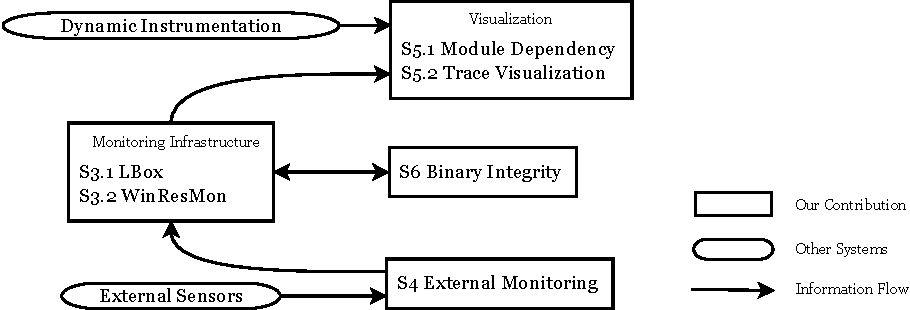
\includegraphics[width=0.8\textwidth]{overview.pdf}
\caption{Overview of the contributions}
\label{fig:overview}
\end{figure}

\TODO{3 parts: monitoring (lbox, winresmon);
software understanding (depvis, lviz);
system security (sensor, binauth)}
